%Préambule du document :
\documentclass[12pt, a4paper]{book}
%\usepackage[latin1]{inputenc} 
\usepackage[utf8]{inputenc} % accents
\usepackage{gensymb} % degree symbol ° (\degree)
\usepackage[T1]{fontenc} % | "`pipe"' character
\usepackage{graphicx}
\usepackage{titling}
\usepackage{amssymb} 
\usepackage{minitoc} % chapter's tocs
\usepackage{authblk} % author affiliations
\usepackage{fancyhdr} % modify the headers
\usepackage{tabularx} % tables not larger than A4
\usepackage[table]{xcolor} %colors inside the tables
\usepackage{float}
\usepackage{multicol} % multiple columns in some sections
\usepackage[inner=2cm,outer=2cm]{geometry} %A4 margins
\usepackage{siunitx}
\usepackage[labelfont=bf, margin=0.5cm]{caption} % for figure captions in minipages
\usepackage{hyperref} %link references (toc, citations) inside document
\usepackage{natbib} % to cite with parentheses and plain text et only year if you please...
\usepackage{amsmath}
 \usepackage{fixltx2e} % allows overrightarrow to be in caption
 \MakeRobust{\overrightarrow}




\bibliographystyle{plainnat} % reference style
\renewcommand{\bibname}{References} %Rename "`bibliography"' => "`references"'

\hypersetup{
    colorlinks,
    citecolor=brown,
    filecolor=green,
    linkcolor=red,
    urlcolor=blue
}
\hypersetup{linktocpage}


\pagestyle{fancy}
\fancyhead{}
\fancyfoot{}
\fancyhead[RO,LE]{\thepage}
\fancyhead[LO]{\leftmark}
\fancyhead[RE]{\rightmark}
\setcounter{tocdepth}{1} % we only want chapters and sections in toc
\setcounter{minitocdepth}{2} %we want sections and subsections in chapters' minitocs

\pretitle{%
  \begin{center}
  
  
\includegraphics[width=17cm]{../Logo_software.png}\\[\bigskipamount]
}
\posttitle{
\\
  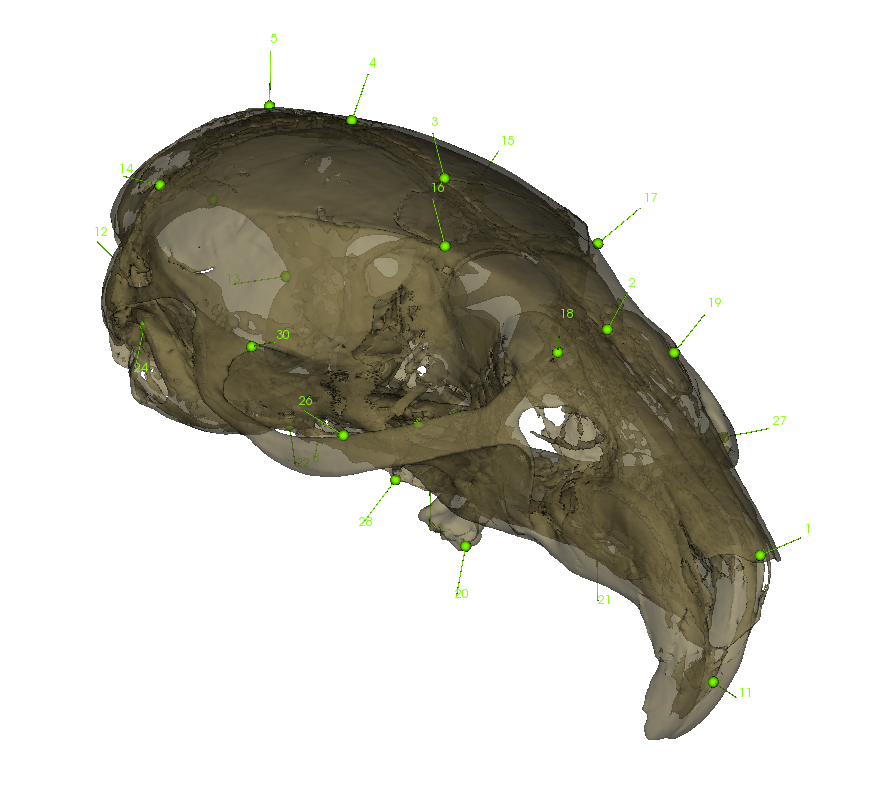
\includegraphics[width=8cm]{tutorial01.png}\\[\bigskipamount]
\end{center}}

%\postdate{
%
\includegraphics[width=15cm]{logo_affiliations.png}
%}

\title{MorphoDig Tutorials\\Tutorial 01: working with landmarks}



%\titlepicture[width=13cm]{Logo_software.png}
\author{Renaud LEBRUN}
\affil{Institut des Sciences de l'Evolution, Université de Montpellier, France}
\date{\today} 

\def\chaptername{Tutorial}
\setcounter{chapter}{0}
%Corps du document :
\begin{document}

	\dominitoc

\maketitle


\tableofcontents

\chapter{Working with landmarks}
\addstarredchapter{Working with landmarks}

\markboth{Working with landmarks}{}

\minitoc 
Tutorial 01 includes:
\begin{itemize}
\item One .ntw (MorphoDig project) file
\item One .vtk surface file representing a cranium of \textit{Mus musculus}
\item One .pos (position) file 
\item One .ori (orientation helper labels) file 
\item One .stv (landmark coordinates and orientation) file
\item The present .pdf document
\end{itemize}





\section{About the specimen}

%\addcontentsline{toc}{section}{About the specimen}
The surface file enclosed in this tutorial represent three-dimensional reconstruction of the cranium of a house mouse (\textit{Mus musculus}) obtained by computerized microtomography at the MRI \si{\micro} CT platform housed at the ISEM.
Before using this tutorial, please download and read MorphoDig User Guide.


\section{A brief overview of enclosed files}
		Download and unzip the files associated to this tutorial. Open MorphoDig.
\subsection{Mouse cranium surface and position files}
	You may open the enclosed .vtk surface file (File -> Surface -> Open Surface, then select "Mouse\_cranium.vtk", or drag and drop this file in the 3D main window). When opened
this way, the corresponding opened surface object is drawn grey, which indicates that this surface
is selected. You may interact with selected objects in different ways (see MorphoDig user guide for
further explanations).\\

By default (\includegraphics[scale=0.7]{../images/06/camera/move_cam2.png}), the camera rotates around the center of mass of all opened objects. This behavior is useful when the center of mass of an object (or of several ones) is far from the origin of the coordinate system. But by pressing the camera button (\includegraphics[scale=0.7]{../images/06/camera/move_cam2.png} -> 
\includegraphics[scale=0.7]{../images/06/camera/move_cam.png}), the camera will revolve around the center of the coordinate system (x=0, y=0, z=0).  The display grid is drawn using different colors depending on the camera rotation center (see Fig. \ref{grid_color} p.\pageref{grid_color}).

\begin{figure}
  \centering
  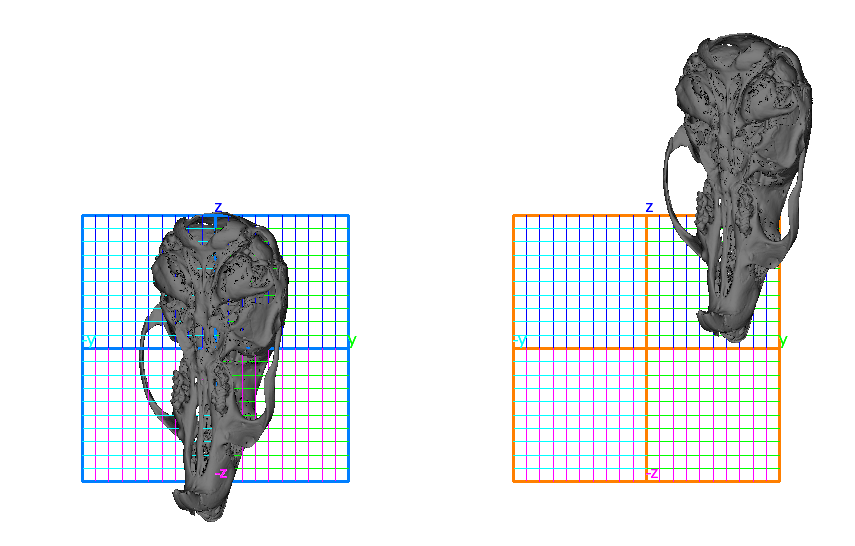
\includegraphics[scale=0.4]{grid.png} 
	\caption{Grid display color.  Left: when the camera revolves around the center of mass of all opened objects, the grid has a blue outline. Right: when the camera revolves around the origin of the coordinate system (x=0, y=0, z=0), the grid outline is displayed in orange.}
\label{grid_color}
 
\end{figure}

 As a general rule, when opening a new object, it is strongly advised to change
its position in order that it matches the 6 predefined camera positions :\\

\includegraphics[scale=0.7]{../images/06/camera/camera_right.png} view object from right side \\

\includegraphics[scale=0.7]{../images/06/camera/camera_left.png} view object from left side\\

\includegraphics[scale=0.7]{../images/06/camera/camera_front.png} view object from front side (default camera position)\\

\includegraphics[scale=0.7]{../images/06/camera/camera_back.png} view object from back side\\

\includegraphics[scale=0.7]{../images/06/camera/camera_above.png} view object from above\\

\includegraphics[scale=0.7]{../images/06/camera/camera_below.png} view object from below\\

In "object interaction mode(
\includegraphics[scale=0.7]{../images/04/move_mode.png})", selected objects can be translated and rotated using the mouse left and middle buttons (in landmark 
\includegraphics[scale=0.7]{../images/04/Landmarks2.png} and camera  
\includegraphics[scale=0.7]{../images/04/camera_mode.png} selection modes, you also need to maintain ``CTRL" button pressed while dragging the left mouse button to achieve rotation and translation of selected objects). Alternatively, you may also use the "yellow sliders" located on the right side of the 3D main window to accomplish rotation and translation of selected objects. Rotation is achieved around the global center of mass of all currently selected objects.\\
\\
The present tutorial contains a .pos (position) file, which you may open in order to place correctly the house
mouse cranium (File -> Position-> Open Position for selected surfaces, then chose "Mouse\_cranium.pos", see Fig. \ref{orientation} p.\pageref{orientation}). If you plan to place landmarks
on internal structures, you may also select the cranium surface (CTRL+A, or drag right mouse button to draw a selection rectangle) and change its transparency (Edit Selected Surface->rendering modifications->Change transparency -> then give a value smaller than 100).\\
All opened surfaces can be unselected by pressing "CTRL +D", or selected by pressing "CTRL +A". All selected objects can be deleted by pressing "Del".

\begin{figure}
  \centering
  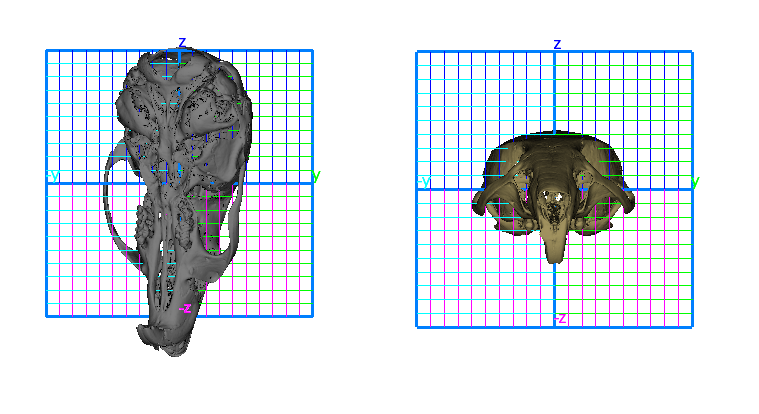
\includegraphics[scale=0.4]{pos.png} 
	\caption{Surface orientation and .POS files.  Left: the mouse cranium positioned in 3D space in the same orientation as it was CT-Scanned. Right: the same cranium in "biologically-relevant" orientation.}
\label{orientation}
 
\end{figure}


\subsection{Mouse cranium project file}
The present tutorial contains a project .ntw file, which may be useful to directly open the mouse
cranium in a convenient position, to make it transparent. First, delete all currently opened objects
(press “CTRL+A”, then press “Del”). Then open the enclosed .ntw file (File->Open Project, then select
“Mouse\_cranium.ntw”). Once loaded, the mouse cranium surface file object is opened, is given the position
enclosed in the “Mouse\_cranium.pos” file, a color and a transparency. Note that the newly opened
surface is unselected.



\subsection{Mouse cranium landmark file}
Prerequisite : make sure that the mouse cranium surface is loaded, and that it is correctly positioned. You
can load the enclosed .stv file (File->Landmarks->Open MorphoDig Landmark/Curve file (.STV)-> Mouse\_cranium.stv or drag and drop this file directly in the 3D main window), which contains 31 landmarks. You can change the way landmarks are rendered in the "Landmark and flag options" window
(Edit->Edit landmark and flag rendering options). You can chose to draw landmarks as spheres or as arrows, and change
their display size. In this tutorial, you may chose to display landmarks as arrows and to let MorphoDig automatically adjust their rendering size.

\subsection{Mouse cranium .ori file}
The present tutorial contains a .ori file, which contains orientation labels for the coordinate system
orientation helper. You can load this file the enclosed .ori file ("File->Orientation helper labels -> Open Orientation labels", then select
"Mouse\_cranium.ori"). Once loaded, the system coordinate orientation helper will show the following
labels :\\
+z axis : dorsal\\
-z axis : ventral\\
+y axis : left\\
-y axis : right\\
+x axis : proximal\\
-x axis : distal\\
You may set your own orientation axis labels with the “Edit orientation labels” window (Viewing opt.-> Orientation labels)

\section{Landmark digitization with MorphoDig}
When setting landmarks, I recommend to press "
\includegraphics[scale=0.7]{../images/04/Landmarks2.png}" to activate the "Landmark mode". When active,
only landmarks can be selected/unselected via right mouse button drag/click. Landmarks can be set
on surfaces by pressing “L” + left mouse click. If a single landmark is selected, its position can be moved
on another part of the surface by pressing “L” + right mouse click (nothing happens if no landmark
is selected or if more than one landmark are selected). Also, you may need to move landmarks away
from the object’s surface (for instance when you want to place a landmark at the centre of a foramen):
once selected, a landmark position can be moved by using the usual mouse (CTRL + middle click + mouse drag) and GUI controls.\\

Two series of conventional landmarks can be set with MorphoDig: "normal" and "target" landmarks.
Press “
\includegraphics[scale=0.7]{../images/04/normal_landmarks.png}” to activate normal landmark setting mode (this mode is active by default), “
\includegraphics[scale=0.7]{../images/04/target_landmarks.png}” to activate target landmark setting mode mode.
You may need to reorder the landmark objects. 
Selected “normal”/”target” landmarks can be reordered
using the following buttons. Clicking on 
\includegraphics[scale=0.7]{../images/06/objects/move_up.png} will increase (= move down in list, if possible) the landmark number of all selected landmarks. Clicking on 
\includegraphics[scale=0.7]{../images/06/objects/move_down.png} will decrease (=move up in list, if possible) the landmark number of all selected landmarks. 

\subsection{Setting landmarks inside the mouse cranium}
Depending on the "z" position of the camera, you may show/hide object, or object parts, which can be useful to set landmarks inside inner structures. You may modify the znear value of the camera by moving the "cp" control = clipping plane slider laying centrally in the left part of the main window (see also Fig. \ref{clipping} p.\pageref{clipping}). You may also use the button 
\includegraphics[scale=0.7]{../images/06/display/cpon.png}/
\includegraphics[scale=0.5]{../images/06/display/cpoff.png}  to adjust / readjust the position of the clipping plane at predefined positions. See MorphoDig User Guide for further explanations. 
\begin{figure}
  \centering
  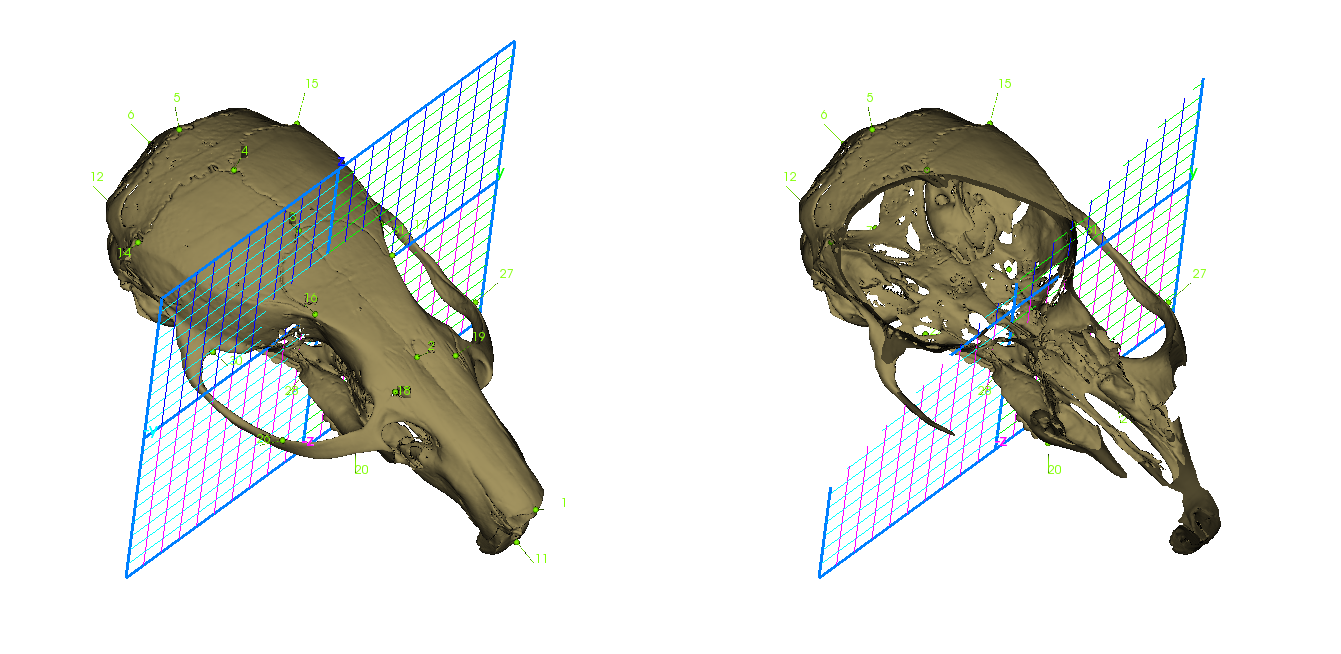
\includegraphics[scale=0.3]{clipping.png} 
	\caption{Clipping plane.  Left: the mouse cranium . Right: the same cranium cut virtually ("cp" slider was moved) in order the visualize inner structures. It is now possible to digitize landmarks inside the the cranium.}
\label{clipping}
 
\end{figure}

\subsection{Saving landmarks}
To save all digitized landmarks, go in "File->Landmarks" and chose the desired option. MorphoDig can manage three types of landmark files: ".LMK", ".VER" and ".STV" files (see MorphoDig user guide for further details).
\subsection{Acknowledgements}
Thanks to the MRI imaging platform for the access to imaging facilities.

%\nocite{*}   % All bibliography items appear without citation in the text

%\cleardoublepage
%\phantomsection

%\addcontentsline{toc}{chapter}{References}
%  \bibliography{References/UsersGuide}		
\end{document} 

